\section{Processing manager}

Processing manager is the major component in the processing of a HLASM source file. It decides which stream of statements is about to be processed and how statements are going to be processed. It contains components responsible for instruction interpretation as well as instruction format validation. 

\begin{figure}
	\centering
	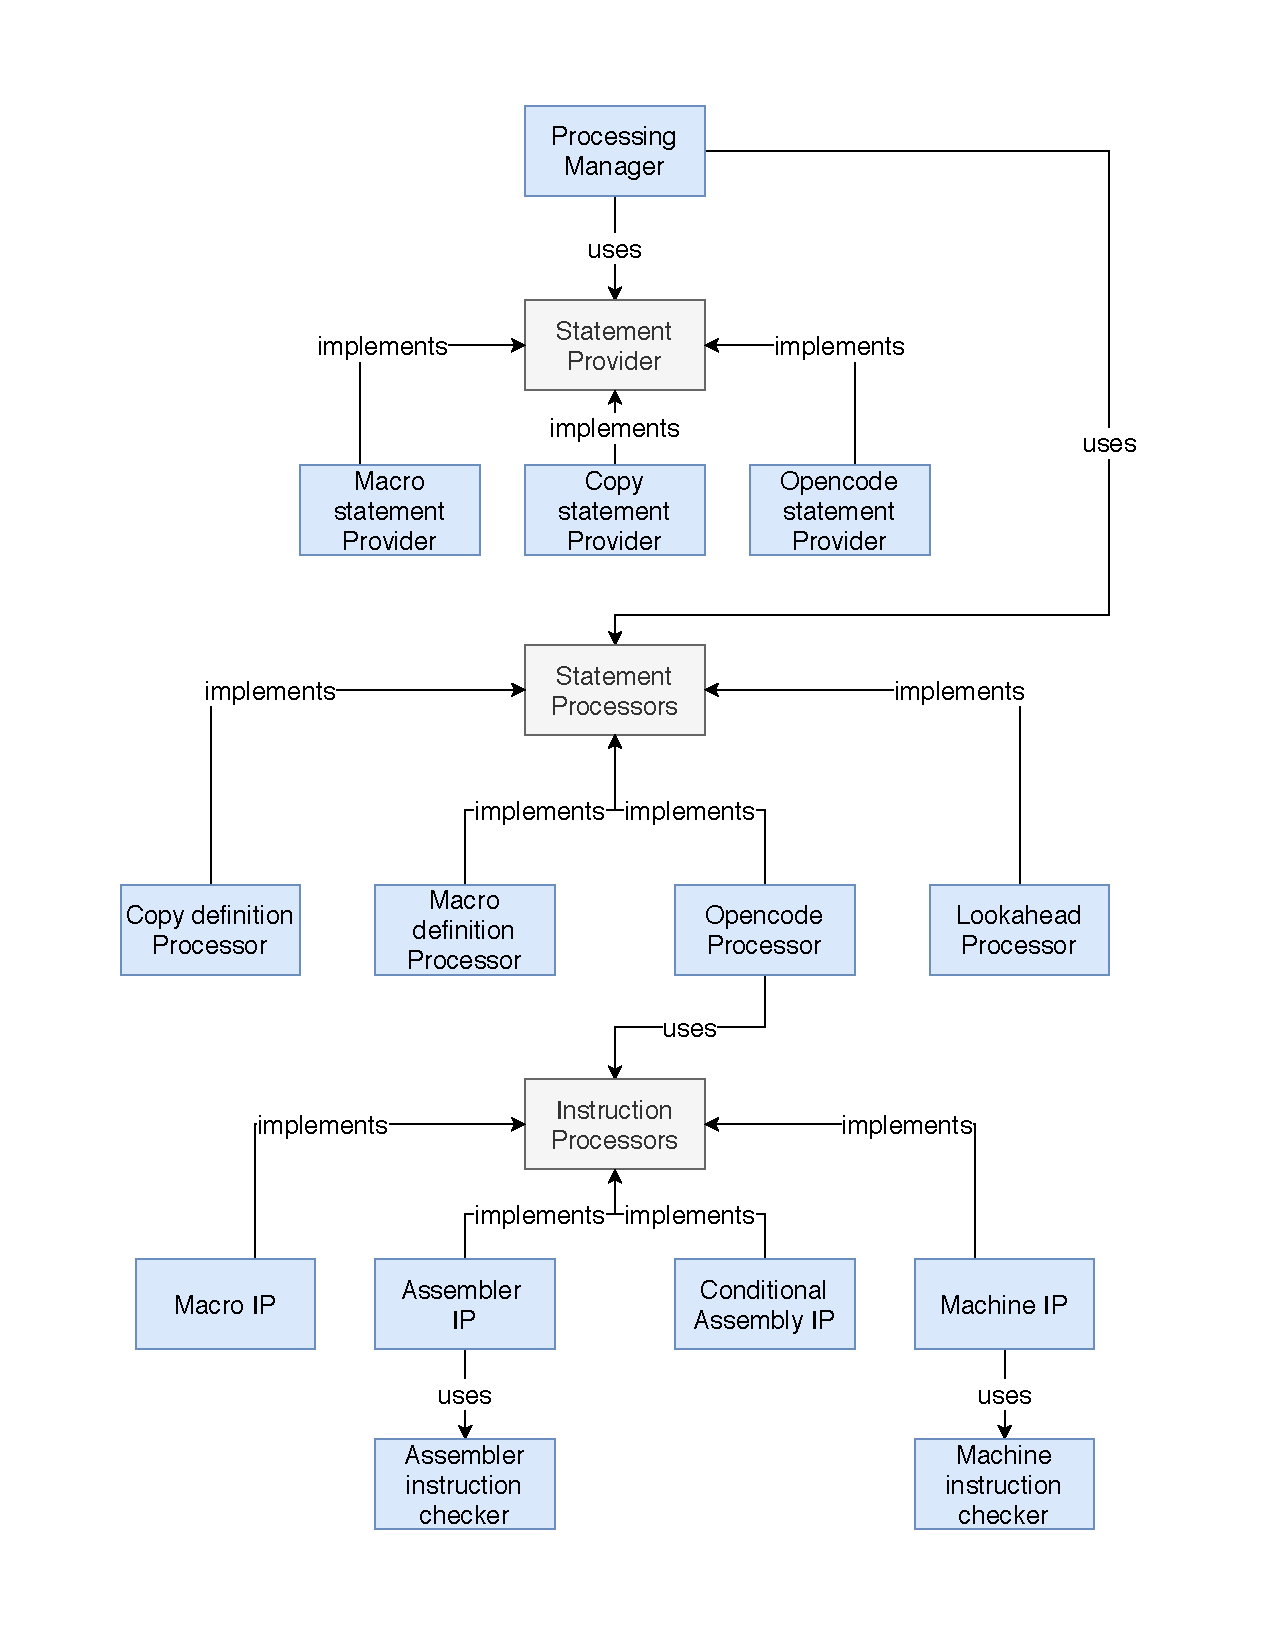
\includegraphics[width=\textwidth]{img/processing_manager_arch}
	\caption{The architecture of Processing manager}
	\label{fig06:proc_mngr}
\end{figure}

\subsection{Overview}

As the processing of the HLASM source file is rather complicated, we define a \emph{statement provider} (see \cref{lab06:sect_prov}) for each different source of statements and a \emph{statement processor} (see \cref{lab06:sect_proc}) for each different manner of statement processing. To lighten functionality of processors, we define \emph{Instruction Processors} (see \cref{lab06:instr_proc}). They focus on different kinds of instructions rather than whole statements. With addition to that, instruction processors use \emph{Instruction format validators}  (see \cref{checker}) that check correct use of the instruction format (see \cref{fig06:proc_mngr}).

Following objects passed by analyzer serve as an input for the processing manager:
\begin{itemize}
	\item \emph{Parser} that provides statements from the processed file. Further on in this chapter, we will refer to the parser as to the \emph{Opencode statement provider}.
	\item \emph{HLASM context tables} that hold current state of the parsed code.
	\item \emph{Library data} defining the initial state of the manager.
	\item \emph{Name} of the processed file.
	\item \emph{Parse library provider} to solve in-file dependencies.
	\item \emph{Statement fields parser} for parsing deferred statements. 
	\item \emph{Processing tracer} for tracing processed statements (see \cref{chap:macro_tracer}).
\end{itemize}

\subsection{Statement Processor}
\label{lab06:sect_proc}


The motivation in distinguishing different statement processors was the complexity of HLASM language. There are many cases when the same statements require different processing under different circumstances (e.g. COPY instruction in macro is handled differently than in opencode, or lookahead mode can accept statements that would fail when processed by ordinary processing).

During processing, kinds of statement processing can be nested. Hence, they are dynamically assigned to the manager when needed and removed from it when they finish.

\subsubsection{Statement}

Statement consists of \emph{statement fields} --- \emph{label field}, \emph{instruction field}, \emph{operands field}, \emph{remark field}. It is used by statement processors and produced by statement providers. 

The abstract class \emph{HLASM statement} is the ancestor for all statement related classes. Then, there are abstract classes \emph{deferred statement} and \emph{resolved statement}. Deferred statement has its operand field stored in uresolved --- deferred --- format (in code stored as string). This statement is created when actual instruction is not yet known prior to the statement creation (see \cref{lst:def_stmt}). Resolved statements are complementary to the deferred statements as their instruction --- as well as operand format --- is known prior to the statement creation.

\begin{listing}[t]
	\begin{verbatim}
*VALUE OF INSTRUCTION IN DEFERRED STATEMENT IS PARAMETER OF MACRO MAC
     MACRO
     MAC      &INSTR
     &INSTR   3(2,0),13      < DEFERRED STATEMENT
     MEND
	\end{verbatim}
	\caption{An example of deferred statement in code.}
	\label{lst:def_stmt}
\end{listing}




\subsubsection{Copy and Macro definition Processors}

Both of these statement processors handle statement collecting, forming definition structure and storing it into HLASM context tables. They come into effect when COPY instruction is encountered in the source code or in the macro definition. 

The statements collected inside copy or macro definitions are mainly deferred statements. That is because variable symbols can not be resolved inside the definition and because HLASM allows instruction aliasing. Therefore, during the processing of a definition, as the instruction field is parsed, the format of its operands is unknown. It is fully deduced when the definition is handed over to the provider and processed by the opencode processor.

However, some statements in the macro and copy definitions forbid aliasing and the operand format can be deduced immediately (e.g. conditional assembly instructions in macro definition). This leads to the processors necessity to ask the provider to retrieve the statement with correct format -- accordingly to the deduced one based on the provided instruction  (see \cref{lab06:proc_stat}).

\subsubsection{Lookahead Processor}
\label{lab06:look}

Lookahead processor is activated when currently processed conditional assembly statement requires a value of undefined ordinary or sequence symbol. It looks through the following statements and finishes when the target symbol is found or when all statement providers finish.

\subsubsection{Opencode Processor}
\label{ord_proc}
Opencode processors (in code described as Ordinary processor) usage can be described in the following points:
\begin{enumerate}
	\item If a model statement is encountered (see \cref{var_sym}), it substitutes the variable symbols and resolves the statement.
	\item Checks statement for validity.
	\item Performs instruction by updating HLASM context tables with the help of \emph{instruction processors}.
\end{enumerate}

It is also passed \emph{processing tracer} by the manager. Each time a statement is processed by opencode processor, it triggers processing tracer. The tracer serves as a listener pattern used by \emph{Macro tracer} (see \cref{chap:macro_tracer}).

\vspace{0.5cm}

During their work, any processor can encounter statement that requires the processor to change (e.g. encountering special instruction or non previously defined sequence symbol, see \cref{tab06:processor_change}). Therefore, they use \emph{processing state listener} interface (implemented by processing manager) that tells the manager to change the current processor.

If we look at the \cref{tab06:processor_change}, we can see that it does not have a field that starts Opencode processor. That is because this processor is set as a default by the manager. The next thing we can see is that Copy processor does not finish itself during its work as it can only be finished by its \emph{terminal condition} (see \cref{tab06:term_cond}). 

Terminal condition can be triggered by a finishing provider. It indicates that the processor needs to finish its work when a specific provider exhausted its statement stream.

\begin{table}
	\centering
	\begin{tabular}{lccccc}
		                   & \thead{\textbf{END}\\ \textbf{instruction}} & \thead{\textbf{COPY}\\ \textbf{instruction}} & \thead{\textbf{MACRO}\\ \textbf{instruction}} & \thead{\textbf{MEND}\\ \textbf{instruction}} & \thead{\textbf{undefined} \\ \textbf{symbol}} \\ \toprule
		\textbf{Opencode}  &                 finish self                 &                 starts Copy                  &                 starts Macro                  &                                              &               starts Lookahead                \\
		\textbf{Copy}      &                                             &                                              &                                               &                                              &                                               \\
		\textbf{Macro}     &                                             &                 starts Copy                  &                                               &                 finish self                  &                                               \\
		\textbf{Lookahead} &                 finish self                 &                 starts Copy                  &                                               &                                              &                                               \\ \bottomrule
	\end{tabular}
	\caption{Description of statement processor changes.}
	\label{tab06:processor_change}
\end{table}

\subsection{Statement Provider}
\label{lab06:sect_prov}

In contrary to statement processors, statement providers are ordered based on the priority (lower index, greater priority):

\begin{enumerate}
	\item Macro definition statement provider
	\item Copy definition statement provider
	\item Opencode statement provider
\end{enumerate}

In each iteration of processing manager (see \cref{lab06:mngr_loop}), providers are asked whether they have statements to provide based on the ordering. That is because after each iteration, a provider with greater priority than the previously used one can be activated. 

\begin{table}
	\centering
	\begin{tabular}{l|ccc}
		\textbf{Processors} & \thead{\textbf{Macro provider} \\ \textbf{ends}} & \thead{\textbf{Copy provider} \\ \textbf{ends}} & \thead{\textbf{Opencode provider} \\ \textbf{ends}} \\ \toprule
		\textbf{Opencode}   &                                                  &                                                 &                     finish self                     \\
		\textbf{Copy}       &                                                  &                                                 &                     finish self                     \\
		\textbf{Macro}      &                   finish self                    &                                                 &                     finish self                     \\
		\textbf{Lookahead}  &                   finish self                    &                                                 &                     finish self                     \\ \bottomrule
	\end{tabular}
	\caption{Description of statement processors' terminal condition.}
	\label{tab06:term_cond}
\end{table}

For the main loop to be correctly defined, opencode provider's end triggers terminal condition for all statement processors. Hence, when opencode provider finishes then all the processors finish as well and the processing ends (see \cref{tab06:term_cond}).

\subsubsection{Statement passing}
\label{lab06:proc_stat}

In HLASM language, it is difficult to parse statements into one common structure due to major differences in operand field of different instruction formats. Moreover, when parsing statements, the instruction format can be yet unknown. Therefore, operand fields are stored as strings. This means that --- during statement passing when instruction format is deduced --- provider has responsibility to produce correct statement format. The following steps are applied in the statement passing (also see \cref{fig06:process_next}):

\begin{enumerate}
	\item Provider retrieves the instruction field part of the statement.
	\item Provider calls processor's \texttt{get\_processing\_status} method with instruction field as a parameter.
	\item Return value of the call determines the required format of the operand field for the processor.
	\item With the return value, provider passes correct statement format to the processor. 
\end{enumerate}

\begin{figure}
	\centering
	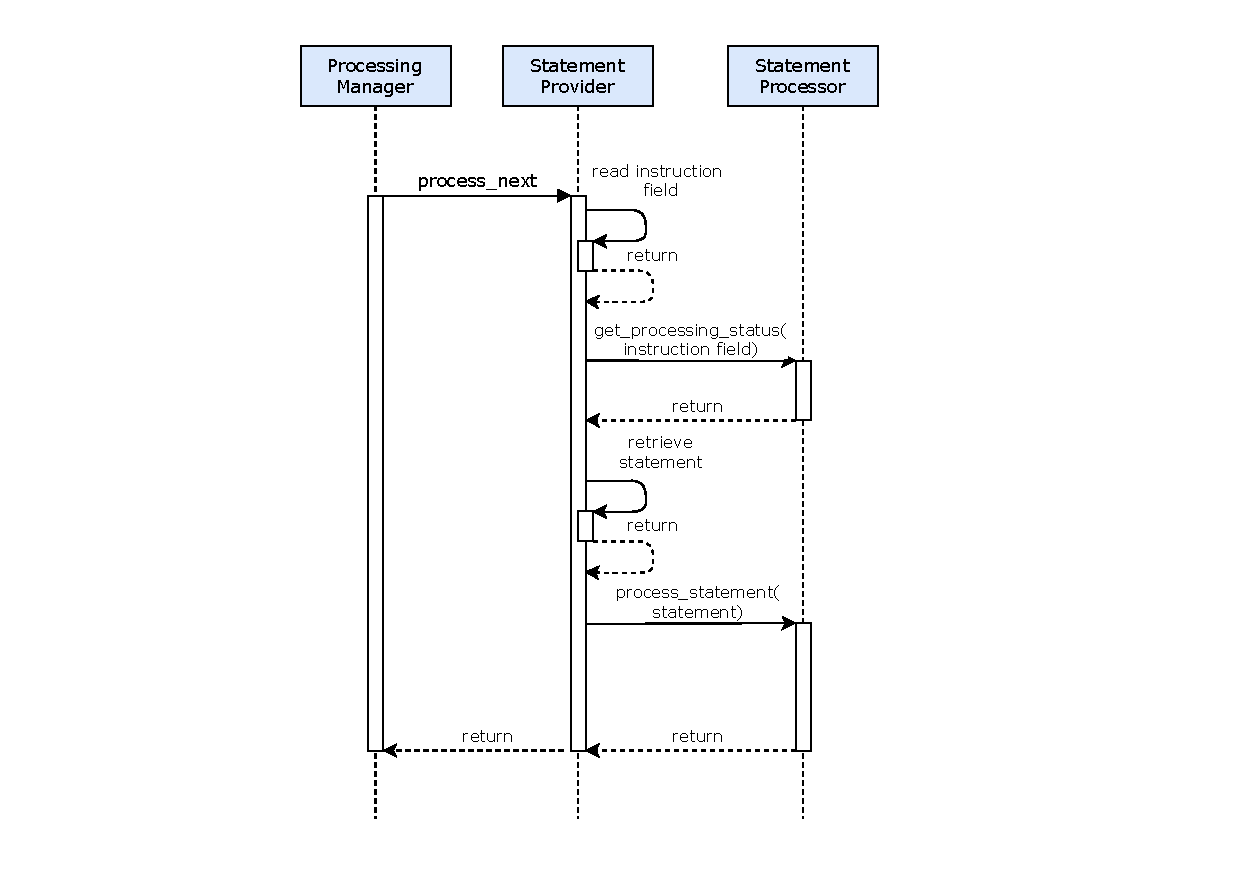
\includegraphics[width=13cm]{img/process_next}
	\caption{The process of statement passing.}
	\label{fig06:process_next}
\end{figure}


\subsubsection{Copy and Macro definition Provider}

These providers are activated when COPY instruction copies a file into the source code or when a macro is visited, respectively. They provide a sequence of statements to an arbitrary processor until all statements from the copy or macro definition are provided. Then, if there is no nested invocation, provider with lower priority is selected.

\subsubsection{Opencode Provider}

Opencode provider is active as long as there are statements in the source file. It retrieves statements from the source code with help of lexer and parser (see \cref{lab06:parser}).

\subsection{The main loop}
\label{lab06:mngr_loop}

Processing manager contains two arrays, each consisting of different instance of statement processor and statement provider respectively.  Also, it has notion of the processor/provider that is in the current use and implement interfaces that swap them.

The main processing loop works with the current processor and provider. In the loop body, as the names suggests, statement provider provides next statement for statement processor that processes it accordingly. The loop breaks when the last processor finishes work.

When provider or processor finishes its work, it is replaced with another. The following rules apply:

\begin{enumerate}
	\item When a processor finishes its work, the next processor is selected from the array.
	\item When a provider finishes --- before the next provider is selected from the array --- manager checks whether it triggers the termination of the current processor as well (\emph{terminal condition}). If true, perform rule 1.
\end{enumerate}

\subsection{The initial state}
\label{lab06:lib_data}
Having described processors and providers, we are ready to talk about which of them are initialized by the manager at the beginning of the processing. The manager determines this from library data passed by analyzer.

Library data contain a file name and enumeration indicating kind of the file that is being parsed --- \emph{processing kind}.

\emph{Ordinary} processing kind states that the file being processed is the main source file (in HLASM called open-code). It is the first file to be processed. With this information, manager initializes all statement providers in respective order and \emph{only} opencode processor. This enumeration is passed when analyzer has owner semantics.

\emph{Copy} and \emph{Macro} processing kinds state that manager will process source code that contains copy or macro definition respectively. Hence, \emph{only} copy definition processor or macro definition processor is initialized. Also, all but macro statement provider are initialized. That is because macro definitions would pollute statement sources (i.e. when parse library provider is called within macro call). Also, no macros will be visited nor needed as a statement source when processing new source code. This enumeration is passed when analyzer has reference semantics.


\subsection{Statement field parser}
\label{lab06:field_parser}

Statement field parser is an interface passed to the statement providers by processing manager implemented by the parser (see \cref{lab06:parser}).

Firstly, it is used during statement passing. In some cases provider is requested a concrete format of a string-stored statement. The string is re-parsed with the according format. Then the field is returned back to the statement provider. 

Another use of field parser is in opencode processor as model statements are resolved there. After variable symbol substitution, the resulting string field is re-parsed with field parser.

\subsection{Instruction processors}
\label{lab06:instr_proc}

Used by ordinary processor, instruction processors are helper classes that divide processing of HLASM instruction types.

As format of some instruction kinds can be rather complicated, instruction processors contain \emph{Instruction format validators} (see \cref{checker}). They check the statement to validate the correctness of used operand format as well as the correctness of the actual operand values.

During the instruction processing, processors encounter HLASM \emph{expressions} (see \cref{ca_expr:logic}, \cref{mach_expr}). They need to be evaluated to correctly perform the processing.

There are four specialized instruction processors:
\paragraph*{Macro IP} looks up for macro definition in HLASM context tables and calls it.
\paragraph*{Assembler and Machine IP} processes assembler and machine instructions (see \cref{asm_instrs} \cref{mach_instr}) to retain consistency in HLASM context tables.

\paragraph*{Conditional assembly IP} executes conditional assembly instructions (see \cref{ca_instr}). 

\vspace{5mm}

See the current list of processed instruction in \cref{tab06:instr_proc}.

\begin{table}
	\centering
	\begin{tabular}{lr}
		\textbf{IP}                   &                  \textbf{Processed instructions} \\ \toprule
		\textbf{Assembler}            & *SECT, COM, LOCTR, EQU, DC, DS, COPY, EXTRN, ORG \\
		\textbf{Machine}              &        \emph{Instruction format validation only} \\
		\textbf{Macro}                &                                       \emph{ANY} \\
		\textbf{Conditional Assembly} &    SET*, GBL*, ANOP, ACTR, AGO, AIF, MACRO, MEND \\ \bottomrule
	\end{tabular}
	\caption{Table of instructions that are processed by instruction processors.}
	\label{tab06:instr_proc}
\end{table}

\subsubsection{CA Expressions}
\label{ca_expr:logic}

HLASM differentiates two kinds of expressions: \emph{Conditional Assembly} (CA) and \emph{Assembler} (ASM) expressions. CA expressions appear in conditional assembly, which is processed during compilation and has a significant impact on the final generated assembly.
On the other hand, assembler instructions are the actual instructions that the processor executes.

In this section, we first describe CA expressions following with ASM instructions.



HLASM evaluates CA expressions during assembly generation. For further details, refer to the \cref{ca_instr}.

We employ the ANTLR 4 Parse-Tree Visitors during the expression evaluation. ANTLR 4 offers two mechanisms for tree-walking: the parse-tree listeners and parse-tree visitors. As the tree-walker encounters a rule, it triggers a \emph{start} function. Similarly, when the walker visits all children of the node, it calls the \emph{finish} function.  The second mechanism is the parse-tree visitor. The visitor lets the programmer control the walk by explicitly calling methods to visit children. We picked the latter approach because we need to have ampler control over the evaluation (such as operator priority).

In this paragraph, we address the representation and functionality of the expressions themselves. Coupling the expressions with grammar and their evaluation in context is further discussed in \cref{ca_expr:eval}.

Each HLASM CA expression has a type. Supported are \emph{arithmetic}, \emph{logic}, \emph{character} expressions. We implement the logic in following classes:

\begin{description}
	\item[\texttt{diagnostic\_op}] Fundamental is the concept of \emph{diagnostics}. During the evaluation of an expression, an error can occur (syntactic or semantic). Hence, we try to improve the user experience by reporting diagnostics. Each instance of \texttt{expression} has a pointer to \texttt{diagnostic\_op} associated. If the pointer is \texttt{null}, it is considered error-free. During the evaluation of a child expression, the parent checks for errors and propagates the error upwards. Checking and propagating of error is implemented by \texttt{copy\_return\_on\_error} macro, which one should call immediately before the creation of new expression during evaluation. For an example see \cref{ca_expr:example}. 
	
	\item[\texttt{expression}] Pure virtual class. It defines the shared interface, operators, and functions. The class also implements evaluation logic for terms and factors. 
	
	The \texttt{expression} class implements the evaluation as follows:
	A \texttt{std::deque} of \texttt{expression} pointers (see  \cref{ca_expr:example}) is passed. The evaluation iterates the list from left to right.  Functions, binary, and unary operators consume the rest of the deque.
	
	Some expression symbols can be either HLASM keywords or variable identifiers. Therefore, the resolution of symbols is complicated and cannot be done straight, but instead during the evaluation-time. The order of the expression's terms and previous evaluation context is crucial for the disambiguation. 
	
	\item[\texttt{keyword\_expression}] Helper class that represents HLASM keywords in expressions. It can decide for a string whether it is a known keyword if its unary or binary operation and what priority it has.
	
	\item[\texttt{logic\_expression}] Represents a logic expression. Note, logic, and arithmetic expression have some common functions, but their behavior differs. 
	
	\item[\texttt{arithmetic\_expression}] Represents an arithmetic expression.
	
	\item[\texttt{arithmetic\_logic\_expr\_wrapper}] HLASM language supports expressions with operands of mixed types. For more straightforward and readable use of arithmetic and logical expression, this class wraps these expression types under one class.
	
	\item[\texttt{character\_expression}] Represents a character expression.
	
	\item[\texttt{ebcdic\_encoding}] This class defines a custom EBCDIC literal and provides helper functions for conversion between EBCDIC and ASCII. EBCDIC is a character encoding used in the IBM mainframe. It has a different layout than ASCII (see \cref{ca_expr:ebcdic}).
	
	\item[\texttt{error\_messages}] It is a static class with list of all \texttt{diagnostic\_op} generated from expressions.
	
	
\end{description}
\begin{lstlisting}[label={ca_expr:example},language=C++,backgroundcolor=\color{cyan!10}, captionpos=b, caption=Defition of \texttt{copy\_return\_on\_error} macro and an example of its usage while evaluating unary expression \texttt{B2A("123")}. \texttt{this} is an \texttt{character\_expression} with value \texttt{"123"}.]
#define copy_return_on_error(arg, type) \
do \
{ \
auto te = test_and_copy_error<type>(arg); \
if (te != nullptr) return te; \
} \
while(0)

//before upward propagating the operation result
//call the macro
copy_return_on_error(this, arithmetic_expression);
return arithmetic_expression::from_string(value_, 2);

\end{lstlisting}

\begin{figure}
	\centering
	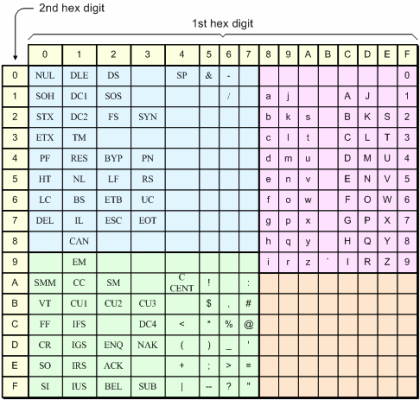
\includegraphics[height=13cm]{img/ebcdic}
	\caption{EBCDIC layout. Taken from \url{https://i.stack.imgur.com/h3u5A.png}.}
	\label{ca_expr:ebcdic}
\end{figure}

\subsubsection{CA expression evaluation}
\label{ca_expr:eval}

In the previous section, we described the representation of the CA expressions themselves. In this section, we explain the coupling of CA expressions with grammar via visitor. 

The \texttt{expression\_evaluator} encapsulates the coupling logic between the grammar and the expression logic. That is, the evaluator has a notion about grammar, which translates into C++ expression logic. At this point, it is essential for the reader to be familiar with the grammar (see \cref{parser:rules}).

The top-level expression first gathers a list of space-separated expressions. We gather this list because a token may be a keyword (such as \texttt{AND} operator) or variable identifier, depending on a position in an expression (using language keywords as identifiers is allowed in HLASM). \texttt{expression::evaluate} provides the disambiguation (see \cref{ca_expr:logic}). 

Evaluator substitutes grammar rules with variable and ordinary symbols for their values and retrieves structure that holds real value of the expression. To know which values to substitute, evaluator is given \emph{evaluation context}. It consists of objects that are required for correct evaluation. It is \emph{HLASM context} for symbol values, \emph{attribute provider} for values of symbol attributes that are not yet defined and \emph{library provider} for evaluation of some types of symbol attributes as well.

In conditional assembly expressions --- when visiting yet not defined ordinary symbol --- lookahead is triggered (see \cref{lab06:look}). As this can be rather demanding operation, expression evaluator uses \emph{expression analyzer}. It looks expression for all the undefined symbol references and collects them to a common collection. Then, lookahead is triggered with requirement of looking for all references of the collection. Hence, it is triggered once each expresssion rather than any time undefined symbol reference is found. 

\subsubsection{Machine expressions}
\label{mach_expr}

In HLASM, machine expressions are used as operands of machine and assembler instructions. Their result may be a simple absolute number or an address.

We use a standard infix tree representation of expressions. There is an interface \TT{machine\_expression} which is implemented by several classes that represent operators and terms. Each binary operator holds two expressions --- left and right operands. Terms are leaf classes that do not hold any other expressions and directly represent a value. There are several classes representing different terms valid in machine expressions:
\begin{itemize}
	\item \TT{mach\_expr\_constant} represents simply a number.
	\item \TT{mach\_expr\_symbol} represents an ordinary symbol.
	\item \TT{mach\_expr\_data\_attr} represents attribute of a symbol (e.g. \TT{L'SYM} is length of symbol \TT{SYM})
	\item \TT{mach\_expr\_location\_counter} represents location counter represented by asterisk in expressions. 
	\item \TT{mach\_expr\_self\_def} represents self defining term (e.g. \TT{X'1F'})
\end{itemize}
\Cref{mach_expr_example} shows an example representation for one concrete expression.

\begin{figure}
	\centering
	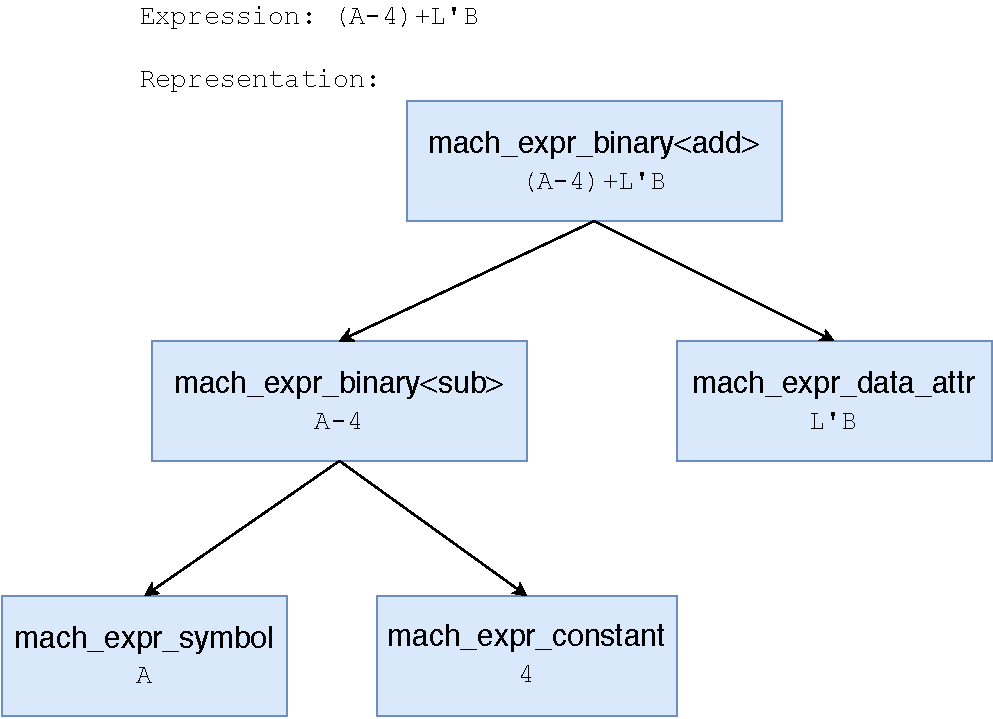
\includegraphics[width=13cm]{img/mach_expr_example}
	\caption{Example of representation of a machine expression}
	\label{mach_expr_example}
\end{figure}

Machine expressions are also able to evaluate the expressions they represent. The evaluation is done in a recursive manner. It is fairly simple when there are no symbols used in the expression --- each node in the tree simply computes the result with basic arithmetic operations.

However, the process can get tricky since expressions may contain e.g. \TT{mach\_expr\_symbol} whose value is dependant on symbols defined in other parts of source code. Moreover, result of a machine expression may be an absolute value (a number) or relocatable value (an address). The process of symbols resolution is explained in \cref{symbol_dependency_tables}.